\chapter{Motivation}
Model Based Engineering an upcoming technology in the domain of electrical and software engineering. In Model Based Engineering the specification of a system is developed as a model.
%The Unified Modelling Language (UML) offers a large set of Modelling Elements and Diagrams and is also extensible. 
%It can be used to describe almost everything. 
One can Model very detailed and describe a System bit by bit and at the same time a simple Diagram can give a quick and intuitive overview over the System. 
Nevertheless %modelling in UML is an effort that needs to pay off to be economic. 
modelling is not an end unto itself. One way to get a benefit from Model Based Engineering is by implementing tool support for many typical engineering tasks. One of those tasks is testing. In Model Based Testing we try to verify an implementation against its specification that is given as a model. It is possible to automatically generate relevant test cases and even working Unit Test code from the Model. In this thesis we are going to develop a tool supporting the generation of Unit Tests from a specification given as UML Model.
\section{A real world problem at Airbus}
\begin{figure}
\label{fig:Act2Code+Tests}
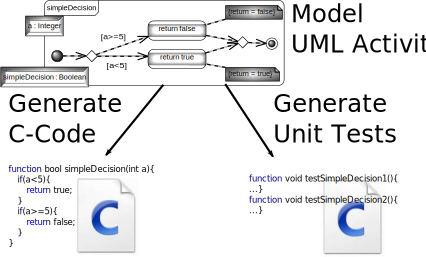
\includegraphics[width=0.7\textwidth]{./pics/Activity2Code+Tests.png}
\caption{Example of an Activity and the generated C-Code and corresponding Unit Tests}
\end{figure}
At Airbus Buxtehude Model Based engineering shall soon replace the traditional requirement driven Engineering approach. There are three main benefits that shall be realized with model based engineering. The first one is that the Model can be used for documentation purpose and several documents required by regulatory bodies can be generated from it. The second is the generation of source code from the model. And the third way to profit from Model Based Engineering is to use the specification as a test model from which all necessary test cases for the software can be deduced.\\
For modelling behaviour and control flow of C functions UML Activities shall be used. The company Atego\textregistered already built a proprietary code generator for Airbus Buxtehude, which generates a folder structure, C source code files and C header files from a UML model and fills function bodies with code generated from UML Activities. The fact that the code is generated does not make it fault free. We still need to validate the generated code by unit tests. The task in this thesis is to build a tool that integrates with the current work flow and can produces the corresponding Unit Tests automatically from the specification.

\section{Idea of this Thesis}
\subsection{Independence of Souce code and Testmodel}
One should not generate the source code as well as the unit test from the same model. We need some independence between the implementation and the corresponding unit tests. Writing the complete unit test code by hand is cumbersome. Generating Unit Tests from a complete new model that is build independently from the model used for code generation still imposes some unnecessary work. The Idea is to share the structure of the Activity between code generation and test generation. While the code generation uses procedural C code snippets that are embedded in the model the test generation only relies on embedded declarative OCL constraints. By using two different programming paradigms as input for code generation and test generation we assure some independence between the generated C-implementation and the unit tests.
\subsection{Mathematical programming for generation of test data}
This thesis focuses on generating unit tests from UML Activities with embedded OCL constraints.
Since there is no tool available fulfilling our needs we decided to use Model transformations to transform the UML Model stepwise into a more precise mathematical Model in which we can generate all necessary input data via constraint solving, mathematical search and optimization. A UML Activity diagram will be transformed into a constraint system. This constraint system can now be solved for any possible path in the Activity. This results in possible input arguments for the C function that will cover the given control flow path. Also all expected return values as well as values for Class properties before and after the execution of the activity will be computed by a mathematical optimization tool. In a last step we are writing the calculated input arguments into a Unit Test code that can be compiled and executed to directly test the given function.

%To be precice at airbus the decicion was to use UML Activities for modelling behavior and controll flow of C functions for embedded Systems. 
%Basically we want to harvest the benefits from Model Based Engineering by building tool support to generate a test suite for a C function. 
%The generated Test Suite should of course be complete according to some coverage criteria to be selected by the user. 
%And it needs to integrate with the currently used Modelling tools. 
%There is no use in having a Tool working with models when you can not use the models from your standard modelling environment but have to build new models. 

%\subsection{Behavioural Modelling}
%\subsection{Generating Unit Tests from Behavioural Model}
%Explain Model Based engineering at Airbus Buxtehude with Component structure of the software and code generation as well as Test generation from a Model.
%Give the short overview over the complete thesis